% \subsubsection{Recolección de la información de los lugares}
% % \label{subs:Los lugares}
%
% En primer lugar se recolectó la información de los lugares que la aplicación contendrá  de forma inicial, al igual que para recolectar las rutas se hizo uso de un \emph{GPS Garmin Nuvi 1300}, el cual cuenta con la opción de guardar locaciones como favoritos, entonces solo fue necesario estar cerca del lugar que se desea guardar y activar esa opción del GPS, este guarda la información en un archivo \emph{.gpx} y con la ayuda de \emph{QGIS} se genero el archivo shapefile correspondiente.\\
%
% Posteriormente es necesario pasar la información geoespacial del shapefile a la base de datos, para esta tarea se hizo uso de una herramienta disponible para postgres, \emph{shp2pgsql}, que permite la conversión de un archivo shapefile a un archivo sql.
%
% % $ shp2pgsql -s 4326 -I -S -c -d ~/Documents/places.shp > places.sql
% \begin{verbatim}
%   $ shp2pgsql -s 3785 -I -S -c -d ~/Documents/places.shp > places.sql
% \end{verbatim}
%
% Con el anterior comando se tiene como resultado un archivo \emph{.sql}, el cual es ingresado en la base de datos ya configurada, de esta forma nuestra base de datos para a contener una tabla geoespacial con datos de tipo \emph{POINT}, los cuales representan los lugares dentro del campus de la UMSS.\\
%
% % \begin{verbatim}
% %   $ shp2pgsql -s 4326 -I -S -c -d ~/Documents/ways.shp > ways.sql
% % \end{verbatim}
% %
% % De la misma forma es necesario pasar la información de las rutas contenidas en un archivo shapefile a un archivo sql, en este caso creará una tabla \emph{WAYS}.\\
%
% El archivo \emph{sql} resultante es usado para popular la base de datos con la información inicial de los lugares que contiene el campus universitario, para tal tarea se usó el siguiente comando.\\
% % Los archivos resultantes \emph{sql} son usados para popular la base de datos .\\
%
% \begin{verbatim}
%   $ psql -d db_ubikate -U db_admin -f /Documents/places.sql
% \end{verbatim}
%
% \begin{figure}[H]
%   \begin{center}
%     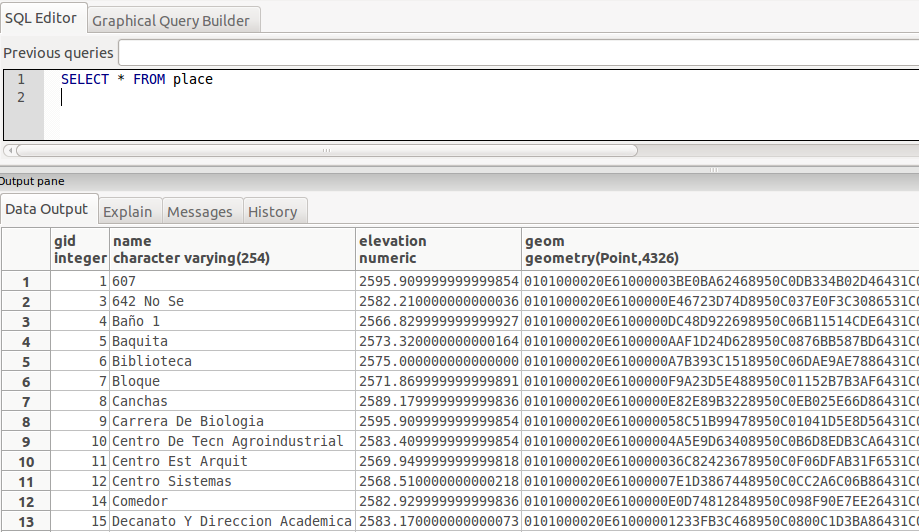
\includegraphics[width=1\textwidth]{iteration1/postgres_places}
%     \caption{Herramienta gráfica de PostgreSQL (\emph{pgAdmin}).}
%     \label{fig:postgres_places}
%     \caption*{Fuente: Elaboración propia}
%   \end{center}
% \end{figure}
%  % con la tabla de Lugares desplegada.
%
% En la figura \ref{fig:postgres_places} se puede observar que la columna \emph{Elevation} contiene datos que el GPS Garmin Nuvi 1300 genera al momento de guardar un punto, en el presente caso es irrelevante.\\
%
%
% Una vez que se tiene populada la base de datos con la información de los lugares es necesario implementar el cómo se comunicara el backend con el frontend, este como ya se explicó se implementará un Servicio Web basado en un API REST.\\

% En la primera Iteración se implementó la lista de lugares que la aplicación mostrará a los usuarios, para lo cual se describe a continuación los pasos que se siguieron. \\


\subsubsection{Acceder a la Información de los lugares mediante un REST API }


La información de un \emph{lugar} está almacenada en una base de datos, entonces para poder acceder a esta información se implementó un REST API, que como ya se especificaron sus características, es la más apropiada para construir una aplicación web. \\

Las peticiones al API llegan a través del protocolo HTTP, en forma de URIs por lo que el servidor implementado con \emph{ExpressJS} tiene que escuchar estas peticiones y actuar en relación al tipo de petición HTTP está llegando, por lo cual es necesario ``mapear'' las URIs con acciones o métodos, como se puede ver en el código \ref{express_api}, los cuales contienen el código necesario para comunicarse con la base de datos. \\


\begin{center}
  \begin{lstlisting}[label=express_api,caption=Declarando API REST con ExpressJS]

        const router = express.Router();
        router.get('/', places.getAll);
        router.get('/:id', places.getPlace);
        router.post('/', places.newPlace);
        router.put('/:id', places.editPlace);
        router.delete('/:id', places.deletePlace);

        app.use('/api/v1/places', router);

  \end{lstlisting}
\end{center}


En realidad, \emph{ExpressJS} no tiene restricciones a la hora de mapear las URIs, pero para una mejor comprensión del API que se está desarrollando, es necesario seguir convenciones que aseguran que cualquier aplicación pueda consumir la información que el API pueda ofrecer, y un REST API cumple con estas características. \\

A cada URI mapeada se lo conoce como \emph{endpoint}, por lo que para obtener la lista de lugares que están registradas en el sistema, se usará el \emph{endpoint}: \verb|router.get('/', places.getAll);|, el cual es el indicado para obtener todos los lugares, según la implementación del REST API visto en la tabla \ref{tab:rest}. \\

El método asociado al \emph{endpoint} contendrá la lógica para comunicarse con la base de datos, por lo que es necesario implementarla. \\


\subsubsection{Implementación de la base de datos para almacenar los lugares}

La característica especial que tiene esta base de datos, es la de manejar datos geoespaciales, en el caso de los \emph{lugares} estos son representados por el tipo POINT.

La base de datos PostgreSQL por defecto no maneja datos geoespaciales, pero como ya se explicó, añadiendo la extensión PostGIS, ya es posible el manejo de datos geoespaciales, pero es nuestra tarea el comprobar que realmente esté manejando los tipos de datos geoespaciales.

Entonces se procedió a recolectar información de un conjunto de lugares, para esta tarea se utilizó un \emph{GPS Garmin Nuvi 1300}, el cual es un dispositivo de posicionamiento global, que cuenta con la opción de guardar locaciones, el dispositivo GPS almacena su información en un archivo \emph{gpx} (que básicamente es un fichero XML estándar usado para compartir datos entre GPS's) y con la ayuda de \emph{QGIS} se gener\'o el archivo shapefile que se utilizó para popular la base de datos con información geoespacial de algunos \emph{lugares} del campus Universitario.

Posteriormente se convierte la información geoespacial almacenada en el shapefile a la base de datos, para lo cual se esta hizo uso de una herramienta propia de PostgreSQL, que permite la conversión de un archivo shapefile a un archivo sql, el cual se puede ver en el siguiente código.

% % $ shp2pgsql -s 4326 -I -S -c -d ~/Documents/places.shp > places.sql
\begin{verbatim}
  $ shp2pgsql -s 3785 -I -S -c -d ~/Documents/places.shp > places.sql
\end{verbatim}

Con el anterior comando se genera un archivo \emph{sql}, el cual es usado para popular la base de datos ya preparada para contener datos geoespaciales, para ingresar la información a la base de datos se utilizó el siguiente comando, propio de PostgreSQL.

% \begin{verbatim}
%   $ shp2pgsql -s 3785 -I -S -c -d ~/Documents/ways.shp > ways.sql
% \end{verbatim}

% % De la misma forma es necesario pasar la información de las rutas contenidas en un archivo shapefile a un archivo sql, en este caso creará una tabla \emph{WAYS}.\\
%
% El archivo \emph{sql} resultante es usado para popular la base de datos con la información inicial de los lugares que contiene el campus universitario, para tal tarea se usó el siguiente comando.\\
% % Los archivos resultantes \emph{sql} son usados para popular la base de datos .\\
%
\begin{verbatim}
  $ psql -d db_ubikate -U db_admin -f /Documents/places.sql
\end{verbatim}

Al finalizar este proceso, se puede ver en la figura \ref{fig:postgres_places}, que la tabla correspondiente a los \emph{lugares} está correctamente populada con la información geoespacial de los lugares registrados con el dispositivo GPS.

\begin{figure}[H]
  \begin{center}
    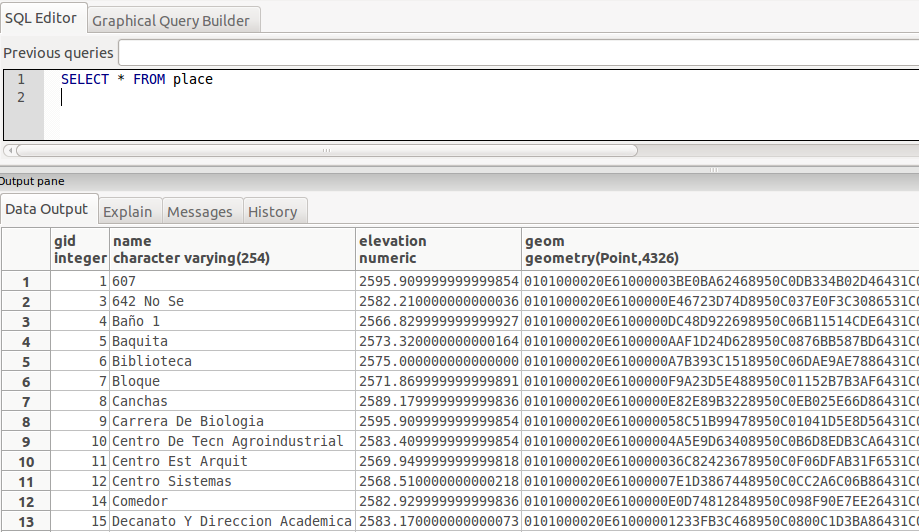
\includegraphics[width=1\textwidth]{iteration1/postgres_places}
    \caption{Herramienta gráfica de PostgreSQL (\emph{pgAdmin}).}
    \label{fig:postgres_places}
    \caption*{Fuente: Elaboración propia}
  \end{center}
\end{figure}
%  % con la tabla de Lugares desplegada.
%
% En la figura \ref{fig:postgres_places} se puede observar que la columna \emph{Elevation} contiene datos que el GPS Garmin Nuvi 1300 genera al momento de guardar un punto, en el presente caso es irrelevante.\\


Una vez implementado el servicio web, necesitamos empezar con el desarrollo del frontend de la aplicación, que como ya se explicó se usará \emph{EmberJS}. \\


\subsubsection{Mostrar la lista de lugares}


\emph{EmberJS} consume la información del API implementado, por lo tanto se hará una llamada \emph{GET} al URI \emph{places/}, que dentro de la estructura de \emph{EmberJS} se tiene que implementar en el \emph{router} dedicado al URI correspondiente. El método mostrado en el código \ref{model_places_index}, es el encargado de hacer generar la petición GET que el API está listo para responder con la lista de los lugares registrados en el sistema. \\

\begin{center}
  \begin{lstlisting}[label=model_places_index,caption=Método para obtener la lista de lugares del API]

    model() {
        var url = (ENV.APP.API_HOST || '') + '/api/v1/places/';
        return jQuery.ajax({
          url: url,
          type: 'GET'
        });
      }

  \end{lstlisting}
\end{center}

Una vez que se obtiene la lista de lugares del servidor, es necesario desplegarlo en el navegador, para tal efecto se implement\'o el método mostrado en el código \ref{template_places_index}, y se utilizó el template correspondiente al URI \emph{templates/places/index.hbs}.

\begin{center}
  \begin{lstlisting}[label=template_places_index,caption=Template de la lista de lugares]

    {{#paper-list}}
      {{#each model.data as |place|}}
        {{#paper-item class="md-1-line" onClick=(transition-to 'places.show' place)}}
            <div class="md-list-item-text">
                <span>{{place.name}}</span>
            </div>
        {{/paper-item}}
        {{paper-divider}}
      {{/each}}
    {{/paper-list}}

  \end{lstlisting}
\end{center}

En la anterior implementación se hizo uso de \emph{ember-paper}, que como ya se explicó ayudará en el \emph{look and feel} de la aplicación, tal como se puede observar en la figura \ref{fig:places_index}. \\
 % tiene toda la apariencia  mejorada para su uso en dispositivos móviles.


\begin{figure}[H]
  \begin{center}
    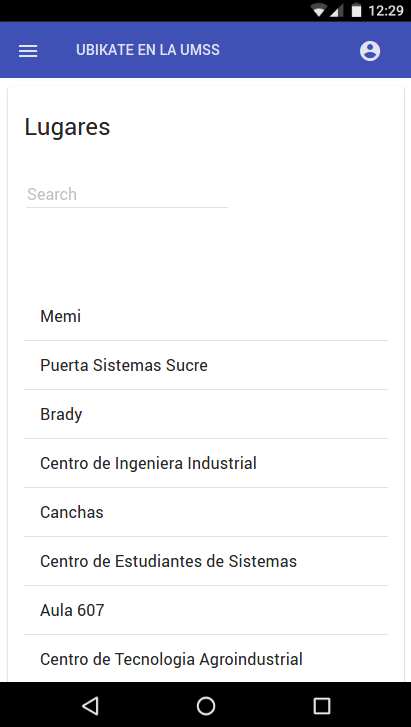
\includegraphics[width=0.3\textwidth]{iteration1/places_index_2}
    \caption{Lista de Lugares}
    \label{fig:places_index}
    \caption*{Fuente: Elaboración propia}
  \end{center}
\end{figure}


\subsubsection{Búsqueda de los lugares}
\label{subs:busqueda de los lugares}

Uno de los criterios de aceptación para la implementación de la \emph{historia de usuario} 2, correspondiente a la búsqueda de los lugares, es que sea posible la búsqueda usando el nombre del lugar o parte del mismo. Al implementar esta \emph{historia de usuario} se a\~nadi\'o un \emph{endpoint} adicional a nuestro servicio web, ver el código \ref{endpoint_search_place}, que basicamente realiza una consulta SQL la cual obtiene de la base de datos los lugares que concuerden con el criterio de búsqueda. \\
 % a continuación se puede ver el URI implementado en la servicio web. \\

\begin{center}
  \begin{lstlisting}[label=endpoint_search_place,caption=Implementación de la búsqueda de lugares en el Servicio Web]

    router.get('places/search/:name', places.getPlacesByName);

  \end{lstlisting}
\end{center}


\subsubsection{Mostrar la información del lugar}
\label{subs:Mostrar información del lugar}

Para mostrar la información de un \emph{lugar}, es necesario realizar una consulta al URI \emph{places/:id} usando el verbo HTTP \emph{GET}, el cual obtiene la información del \emph{lugar} en formato JSON la cual es mostrarda en el navegador, para tal efecto se emplea el template correspondiente al URI,  \emph{app/templates/places/show}, la implementación del template se puede ver en el código \ref{template_places_show}. \\

\newpage
\begin{center}
  \begin{lstlisting}[label=template_places_show,caption=Template para mostrar la información de un lugar]

      {{#text.headline}}{{model.name}}{{/text.headline}}
      {{#card.content}}
          {{#paper-list}}
              {{model.description}}
              {{/paper-item}}
                  {{paper-icon "local_phone"}} {{model.phone}}
              {{/paper-item}}
              {{#paper-item class="md-2-line" }}
                  {{paper-icon "layers"}} Piso N# {{model.level}}
              {{/paper-item}}
          {{/paper-list}}
      {{/card.content}}

  \end{lstlisting}
\end{center}

El resultado en el navegador del template implementado se puede apreciar en la figura \ref{fig:place_show}. \\

\begin{figure}[H]
  \begin{center}
    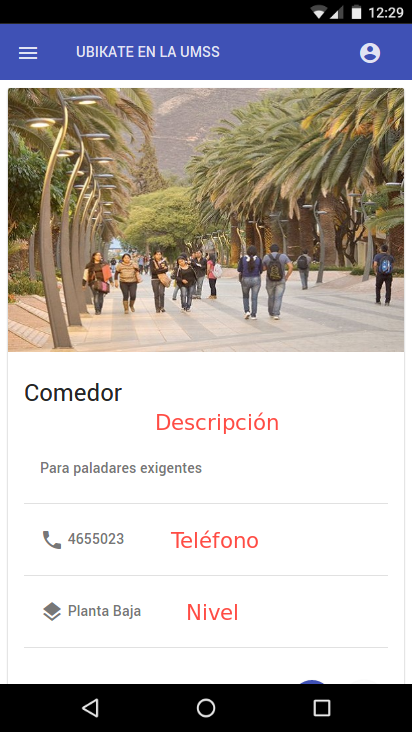
\includegraphics[width=0.3\textwidth]{iteration1/place_show}
    \caption{Vista de la Información de un Lugar.}
    \label{fig:place_show}
    \caption*{Fuente: Elaboración propia}
  \end{center}
\end{figure}




% En la figura \ref{fig:places_index}, se puede observar un
